\section{Perspective Projection}%
\label{sec:perspective_projection}


\subsection{Historic Remarks}%
\label{sub:historic_remarks}


\begin{figure}[h]
\centering
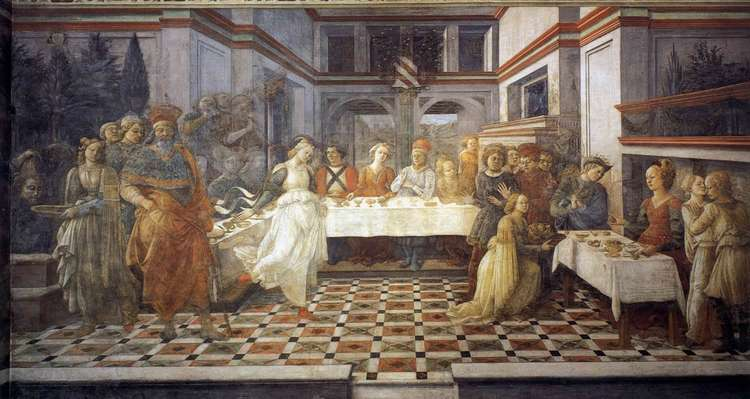
\includegraphics[width=\columnwidth]{img/lippi_feast_herod.jpg}
\caption{Filippo Lippi, ``The Feast of Herod: Salome's Dance.''
Fresco, Cappella Maggiore, Duomo, Prato, Italy, c.1460--1464.}%
\label{fig:lippi_feast_herod}
\end{figure}

\begin{figure}[h]
\centering
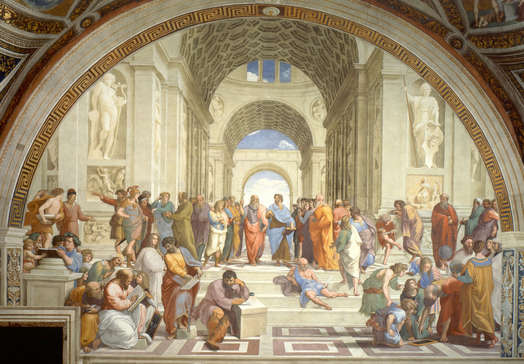
\includegraphics[width=\columnwidth]{img/raphael_school_athens.jpg}
\caption{Raphael, The School of Athens (1509)}%
\label{fig:raphael_school_athens}
\end{figure}

\begin{figure}[h]
\centering
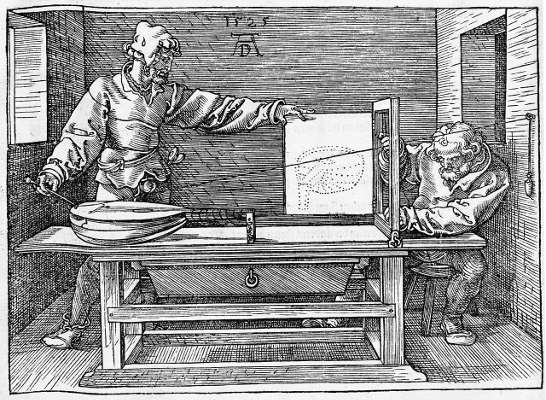
\includegraphics[width=\columnwidth]{img/durer_perspective_machine.jpg}
\caption{D\"urer's perspective machine (1525)}%
\label{fig:durer_perspective_machine}
\end{figure}

The study of the image formation process has a long history.
The earliest formulations of the geometry of image formation
can be traced back to \textbf{Euclid} (4th century B.C.).
Examples of a partially correct \textbf{perspective projection}
are visible in the \textbf{frescoes and mosaics of Pompeii} (1 B.C.).\\

These skills seem to have been lost with the fall of the Roman empire.
Correct perspective projection emerged again around 1000 years later
in early \textbf{Renaissance art}.\\

Among the proponents of perspective projection are the
Renaissance artists \textbf{Brunelleschi, Donatello} and \textbf{Alberti}.
The first treatise on the projection process, \textbf{``Della Pittura''},
was published by \textbf{Leon Battista Alberti}.\\

Appart from the geometry of image formation, the study of the
interaction of light with matter was propagated by artists like
\textbf{Leonardo da Vinci} in the 1500s and by Renaissance painters
such as \textbf{Caravaggio} and \textbf{Raphael}.\\

In Figure~\ref{fig:lippi_feast_herod} and Figure~\ref{fig:raphael_school_athens}
the perspective emerges from the vanishing point.

\begin{figure}[h]
\centering
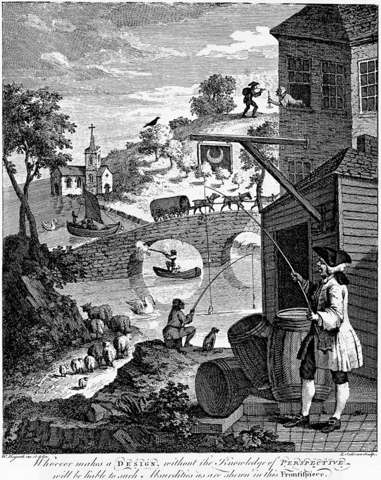
\includegraphics[width=\columnwidth]{img/hogarth_satire.jpg}
\caption{Satire by Hogarth 1753}%
\label{fig:hogarth_satire}
\end{figure}

\begin{figure}[h]
\centering
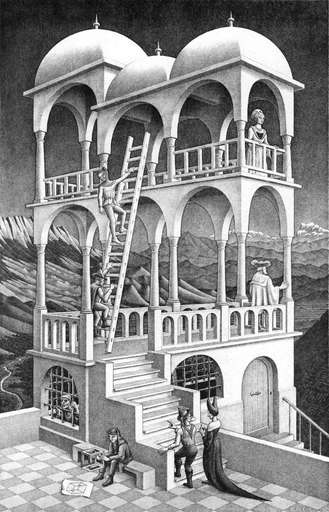
\includegraphics[width=\columnwidth]{img/escher_belvedere.jpg}
\caption{Escher, Belvedere 1958}%
\label{fig:escher_belvedere}
\end{figure}

D\"urer devised a machine to get a perspectively correct image,
see Figure~\ref{fig:durer_perspective_machine}.
It is a manual reproduction of what a camera does today.\\

Many artists played with those perspective rules to create images
that seems locally correct but have inconsitent depth or gravity, like
in Figures~[\ref{fig:hogarth_satire},\ref{fig:escher_belvedere}].


\subsection{Mathematical Representation}%
\label{sub:mathematical_representation}


\begin{figure}[h]
\centering
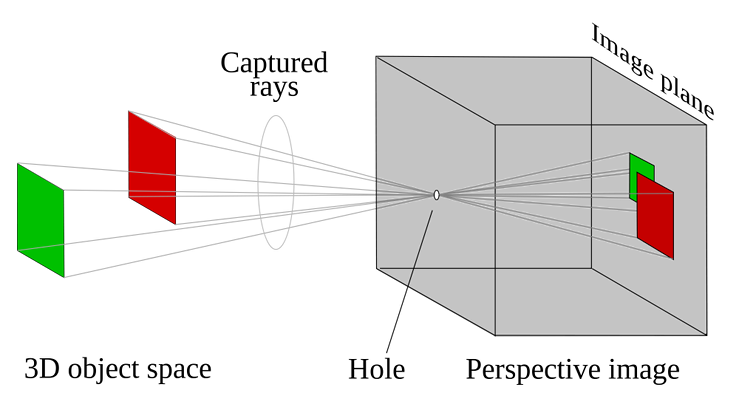
\includegraphics[width=\columnwidth]{img/pinhole_camera.png}
\caption{Pinhole camera model}%
\label{fig:pinhole_camera}
\end{figure}

\begin{figure}[h]
\centering
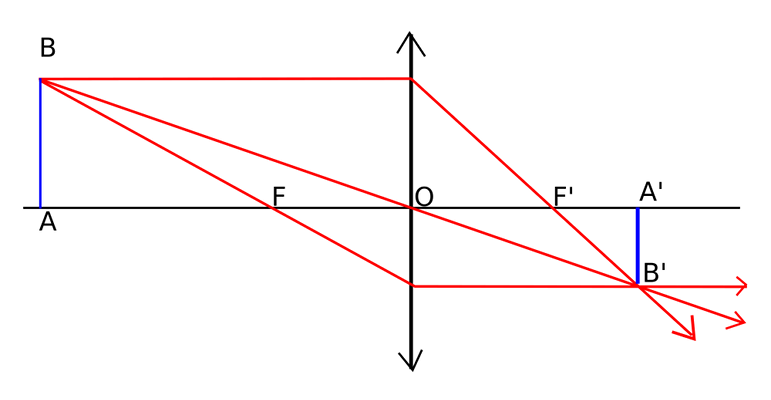
\includegraphics[width=\columnwidth]{img/convex_lense.png}
\caption{Thin convex lense model}%
\label{fig:convex_lense}
\end{figure}

Perspective projection emerges by the so-called pinhole camera model
(see Figure~\ref{fig:pinhole_camera}).
It's main issue is that the hole has to be very small,
perventing light to enter the capture device.
In order to augment the the amount of light we use lenses\\

As visible in (Figure~\ref{fig:convex_lense}), the image is upside down
in the image plan. In order to avoid dealing with minus signs in the
equations, we pretend that the image plan is virtually on the same
side than the object. The perspective thansformation $\pi$ is given by
\[ \pi : \R^3 \rightarrow \R^2; \quad
	\bm{X} \mapsto x = \pi(\bm{X}) =
	\begin{pmatrix}
		f \frac{X}{Z} \\
		f \frac{Y}{Z} \\
	\end{pmatrix}
\]
Where $f$ is the focal length, $X,Y,Z$ are the object coordinates
in the 3D world, the $z$ axis being the camera axis.
The one challenge we have to overcome, is that this transformation is non linear.\\

In order to do so, we will use \textbf{homogeneous coordinates},
which is basically similar to multiplying everything by $Z$:
\[ Z \bm{x} = Z \begin{pmatrix} x \\ y \\ 1 \end{pmatrix} =
	\begin{pmatrix}
		f & 0 & 0 & 0 \\
		0 & f & 0 & 0 \\
		0 & 0 & 1 & 0 \\
	\end{pmatrix}
	\begin{pmatrix}
		X \\ Y \\ Z \\ 1
	\end{pmatrix}
	= K_f \Pi_0 \bm{X}
\]
Where we have introduced the two matrices
\[K_f \equiv
	\begin{pmatrix}
		f & 0 & 0 \\
		0 & f & 0 \\
		0 & 0 & 1 \\
	\end{pmatrix}
	\quad \text{and} \quad
	\Pi_0 \equiv
	\begin{pmatrix}
		1 & 0 & 0 & 0 \\
		0 & 1 & 0 & 0 \\
		0 & 0 & 1 & 0 \\
	\end{pmatrix}
\]
The matrix $\Pi_0$ is referred to as the \textbf{standard projection matrix}.
A first order approximation can consider that all object points
are approximately at the same distance $\lambda > 0$. Thus we obtain:
\[\lambda \bm{x} = K_f \Pi_0 \bm{X}\]

We know that due to the \textbf{rigid motion of the camera},
the point $\bm{x}$ \textbf{in camera coordinates} is given as a function
of the point in \textbf{wold coordinates} $\bm{X}_0$ by:
\[\bm{X} = R \bm{X}_0 + T\]
or in homogeneous coordinates:
\[\bm{X} = g \bm{X}_0 = \begin{pmatrix}R & T \\ 0 & 1\end{pmatrix} \bm{X}_0\]
In total, the transformation from world coordinates to image coordinates
is therefore given by:
\[\boxed{\lambda\ \bm{x} = K_f\ \Pi_0\ g\ \bm{X}_0}\]


\subsection{Intrinsic Parameters}%
\label{sub:intrinsic_parameters}


If the camera is not centered at the optical center, we have an additional
translation $o_x, o_y$. The point were the optical axis intersects
the image plan is called the \textbf{principal point}.\\

If pixels do not have unit scale, we need to introduce
additional scaling factors $s_x$ and $s_y$.
If pixels are not rectangular, we also have a \textbf{skew factor} $s_{\theta}$.\\

The transformation from initial real world coordinates to final pixel coordinates
follows the following steps:
World (3D, $\bm{X}_0$) $\mapsto$ Camera (3D, $\bm{X}$)
$\mapsto$ Image (2D, $\bm{x}$) $\mapsto$ Pixel (2D, $\bm{x'}$).\\

The pixel coordinates $\bm{x'} = (x',y',1)$ are given by:
\[\lambda \begin{pmatrix}x' \\ y' \\ 1\end{pmatrix} =
	K_s\ K_f\ \Pi_0
	\begin{pmatrix}X \\ Y \\ Z \\ 1\end{pmatrix}
\]
where
\[K_s = \begin{pmatrix}
		s_x & s_{\theta} & o_x \\
		0 & s_y & o_y \\
		0 & 0 & 1 \\
	\end{pmatrix}
	\quad K_f =
	\begin{pmatrix}
		f & 0 & 0 \\
		0 & f & 0 \\
		0 & 0 & 1 \\
	\end{pmatrix}
\]
We call $K = K_s\ K_f$ the \textbf{intrinsic parameter matrix}.\\

Therefore, as a function of world coordinates, we have:
\[\boxed{ \lambda\ \bm{x'} = \Pi\ \bm{X}_0
	= K\ \Pi_0\ g\ \bm{X}_0}
\]
The $3 \times 4$ matrix $\Pi$ is called a \textbf{general projection matrix}.
If we get rid of $\lambda$ we obtain the following coordinates:
\[ x' = \frac{\tr{\pi_1} \bm{X}_0}{\tr{\pi_3} \bm{X}_0},\quad
 y' = \frac{\tr{\pi_2} \bm{X}_0}{\tr{\pi_3} \bm{X}_0},\quad
 z' = 1
\]
where $\tr{\pi_1}, \tr{\pi_2}, \tr{\pi_3} \in \R^4$
are the three rows of the projection matrix $\Pi$.


\subsection{Spherical Projection}%
\label{sub:spherical_projection}


The perspective pinhole camera introduced previously considers a planar
imaging suface. Instead, one can consider a spherical projection surface
given by the unit sphere
\[\mathbb{S}^2 \equiv \Set{x \in \R^3}{\|x\| = 1}\]
The \textbf{spherical projection} of a 3D point $\bm{X}$ is given by:
\[\pi_s : \R^3 \rightarrow \mathbb{S}^2;\quad
	\bm{X} \mapsto \bm{x} = \frac{\bm{X}}{\bm{|X|}}\]

The pixel coordinates $\bm{x}'$ as a function of the world coordinates
$\bm{X}_0$ are:
\[
	\lambda\ \bm{x}' = K\ \Pi_0\ g\ \bm{X}_0
\]
except that the scalar factor is now $\lambda = |\bm{X}|
= \sqrt{ X^2 + Y^2 + Z^2 }$.


\subsection{Radial Distortion}%
\label{sub:radial_distortion}


\begin{figure}[h]
\centering

\includegraphics[width=\columnwidth]{img/barrel_distortion.png}
\caption{Grid projection with radial distortion.}%
\label{fig:radial_distortion}
\end{figure}

The intrinsic parameters in the matrix $K$ model linear distortions
in the transformation to pixel coordinates.
In practice however, one can also encounter significant
\textbf{distortions along the radial axis}~[\ref{fig:radial_distortion}],
in particular in a wide field of view is used or if one uses cheaper cameras
such as webcams.
A simple effective model for such distortions is:
\[
	x = x_d ( 1 + a_1 r^2 + a_2 r^4 ),
	y = y_d ( 1 + a_1 r^2 + a_2 r^4 )
\]
where $\bm{x} \equiv (x_d, y_d)$ is the distorted point,
$r^2 = \|\bm{x}\|^2$.
Usually, $a_1$ and $a_2$ are estimated through a calibration step.\\

Other more sophisticated models exist (Devernay and Faugeras '95).
Parameters are computed from
\textbf{distortions of staight lines} (see Figure~\ref{fig:radial_distortion})
or \textbf{simultaneously with the 3D reconstruction}
(Zhang '96, Stein '97, Fitzgibbon '01).


\subsection{Preimage and Coimage}%
\label{sub:preimage_and_coimage}


Due to the unknown scale factor, each point is mapped not to a single
point $\bm{x}$, but to an \textbf{equivalence class of points} $\bm{ y \sim x}$.
It is therefore useful to \textbf{study how lines are transformed}.
A line $L$ in 3-D is characterized by a base point
$\bm{X}_0 = \tr{(X_0, Y_0, Z_0, 1)} \in \R^4$ and a vector
$\bm{V} = \tr{(V_1, V_2, V_3, 0)} \in \R^4$ such that:
\[
	\bm{X} = \bm{X}_0 + \mu \bm{V}, \quad \mu \in \R
\]
The image of the line $L$ is given by:
\[
	\bm{x} \sim \Pi_0 \bm{X}
	= \Pi_0 ( \bm{X}_0 + \mu \bm{V} )
	= \Pi_0 \bm{X}_0 + \mu \Pi_0 \bm{V}
\]
All points $\bm{x}$ treated as vectors from the origin $o$ span a 2-D
subspace $P$. The intersection of this plane $P$ with the image plane
gives the image of the line.
$P$ is called the preimage of the line.
A \textbf{preimage of a point or a line} in the image plane
is the largest set of 3D points that give rise to an image
equal to the given point or line.\\

In case of points and lines, the preimage is a subspace of $\R^3$.
This subspace can also be represented by its orthogonal complement.
This complement is called the coimage.
The \textbf{coimage of a point or a line} is the subspace in $\R^3$
that is the (unique) orthogonal complement of its preimage.\\

\begin{tabular}{ll}
	image &$=$ preimage $\cap$ image plane,\\
	preimage &$=$ span (image),\\
	coimage &$=$ preimage$^{\bot}$,\\
\end{tabular}\\[1em]

In the case of a line $L$, the coimage can be characterized by
a vector $l$ such that:
\[
	\tr{l} \bm{x} = 0
\]
In summary we have the table~\ref{tab:expression_preimage_coimage}:

\begin{table}[h]
\small
\begin{tabular}{cccc}
	& Image & Preimage & Coimage \\ \midrule
	Point
		& $\text{span}(\bm{x}) \cap$ im.\,plane
		& $\text{span}(\bm{x})$
		& $\text{span}(\bm{\widehat{x}})$ \\
	Line
		& $\text{span}(\widehat{l}) \cap$ im.\,plane
		& $\text{span}(\widehat{l})$
		& $\text{span}(l)$ \\
\end{tabular}
\caption{Expression of preimage and coimage}%
\label{tab:expression_preimage_coimage}
\end{table}



\subsection{Projective Geometry}%
\label{sub:projective_geometry}


In order to formally write transformations by linear operations,
we made extensive use of \textbf{homogeneous coordinates} to represent
3D point as a 4D-vector $(X,Y,Z,1)$ with the last coordinate fixed to 1.
This normalization is not always necessary. One can represent 3D points
by a general 4D vector:
\[
	\bm{X} = (XW, YW, ZW, W)\ \in\ \R^4
\]
In general, an \textbf{n-dimensional projective space} $\mathbb{P}^n$
is the set of all one-dimensional subspaces (i.e.\ lines through the origin)
of the vector space $\R^{n+1}$.
A point $p \in \mathbb{P}^n$ can then be assigned homogeneous coordinates
$\bm{X} = \tr{(x_1, \ldots, x_{n+1})}$, among which at least one $x$ is nonzero.
For any nonzero $\lambda \in \R$, the coordinates
$\bm{Y} = \tr{(\lambda x_1, \ldots, \lambda x_{n+1})}$
represent the same point $p$.
